\section{RUIMTEMEETKUNDE} \label{ruimtemeetkunde}
\hypertarget{ruimtemeetkunde}{}

\subsection{Inhoud en oppervlakte van ruimtefiguren} \label{inhoud_ruimtefiguren}
\hypertarget{inhoud_ruimtefiguren}{}

\subsubsection{Prisma} \label{prisma}
\hypertarget{prisma}{}
Stel $G$ de oppervlakte van het grondvlak.\newline
%\docLink[tekening]{prisma.jpg}{\includegraphics{tekening.gif}}\newline
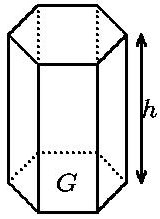
\includegraphics{prisma.jpg}
$I=G\cdot h$

\subsubsection{Piramide} \label{piramide}
\hypertarget{piramide}{}
Stel $G$ de oppervlakte van het grondvlak.\newline
%\docLink[tekening]{piramide.jpg}{\includegraphics{tekening.gif}}\newline
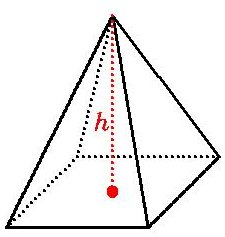
\includegraphics{piramide.jpg}
$I=\ds\Frac{1}{3}G\cdot h$

\subsubsection{Cilinder} \label{cilinder}
\hypertarget{cilinder}{}
%\docLink[tekening]{cilinder.jpg}{\includegraphics{tekening.gif}}\newline
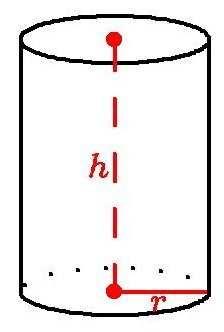
\includegraphics{cilinder.jpg}
$I=\pi r^2 h$\newline
De zijdelingse oppervlakte van een rechte cilinder: $O = 2\pi r h $

\subsubsection{Kegel} \label{kegel}
\hypertarget{kegel}{}
%\docLink[tekening]{kegel.jpg}{\includegraphics{tekening.gif}}\newline
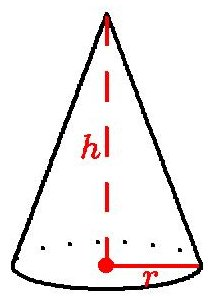
\includegraphics{kegel.jpg}
$I=\ds\Frac{1}{3}\pi r^2 h$\newline
De zijdelingse oppervlakte van een rechte kegel: $O = \pi r \sqrt{h^2+r^2}$

\subsubsection{Bol} \label{bol}
\hypertarget{bol}{}
%\docLink[tekening]{bol.jpg}{\includegraphics{tekening.gif}}\newline
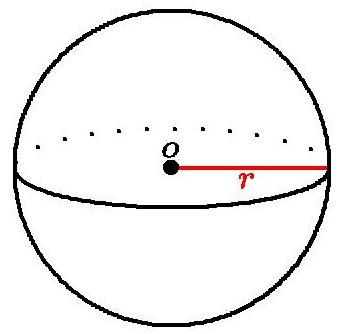
\includegraphics{bol.jpg}
$I=\ds\Frac{4}{3}\pi r^3$\newline
De oppervlakte: $O = 4\pi r^2$

\subsection{Vectoren}
Zie hoofdstuk over vectoren in Sectie~\ref{vectoren} op pagina~\pageref{vectoren}.

\subsection{Co\"ordinaten in de ruimte} \label{coordinaten_in_de_ruimte}
\hypertarget{coordinaten_in_de_ruimte}{}

\subsubsection{Richtingsvectoren-richtingsgetallen} \label{richtingsgetallen}
\hypertarget{richtingsgetallen}
\[\vec{pq} \,\mbox{is een {\bf richtingsvector} van de rechte}\, A \,\Leftrightarrow\, pq \| A\]
\vskip 0.5cm
\begin{center}
De co\"ordinaat van een richtingsvector van A noemen we een stel {\bf richtingsgetallen} van A.
\end{center}
\vskip 0.5cm
{\bf Voorbeeld:} \newline Zij $p(x_1, y_1, z_1)$ en $q(x_2, y_2, z_2)$ twee punten gelegen op de rechte A.\newline Dan is $\vec{pq}$ een richtingsvector van A en is co$(\vec{pq})=(x_2-x_1, y_2-y_1, z_2-z_1)$ een stel richtingsgetallen van $A$.

\subsubsection{Vergelijkingen van een rechte} \label{vergelijking_rechte}
\hypertarget{vergelijking_rechte}{}
\begin{itemize}
\item[*] Rechte bepaald door punt en richtingsvector:\vskip 0.5cm
Zij $p(x_1, y_1, z_1)$ een punt van de rechte en $\vec{q}(a_1, b_1, c_1)$ een richtingsvector, dan zijn de {\bf parametervergelijkingen}:
\begin{eqnarray*}
x & = & x_1 +ra_1 \\
y & = & y_1 +rb_1 \\
z & = & z_1 +rc_1 \\
\end{eqnarray*}
en de {\bf Cartesiaanse vergelijkingen }: 
\[\ds\Frac{x-x_1}{a_1}=\Frac{y-y_1}{b_1}=\Frac{z-z_1}{c_1}\]\vskip 0.5cm
\item[*] Rechte bepaald door twee punten:\vskip 0.5 cm
Zij $p(x_1, y_1, z_1)$ en $q(x_2, y_2, z_2)$ twee punten van de rechte, dan zijn de {\bf parametervergelijkingen}:
\begin{eqnarray*}
x=x_1+r(x_2-x_1)\\
y=y_1+r(y_2-y_1)\\
z=z_1+r(z_2-z_1)\\
\end{eqnarray*}
en de {\bf Cartesiaanse vergelijkingen}: 
\[\ds\Frac{x-x_1}{x_2-x_1}=\Frac{y-y_1}{y_2-y_1}=\Frac{z-z_1}{z_2-z_1}\]
\end{itemize}

\subsubsection{Vergelijking van een vlak} \label{vergelijking_vlak}
\hypertarget{vergelijking_vlak}{}
\begin{itemize}
\item[*] Vlak bepaald door een punt en twee onafhankelijke richtingsvectoren:\vskip 0.5 cm
Zij $p(x_1, y_1, z_1)$ een punt en $\vec{q}(a_1, b_1, c_1)$ en $\vec{r}(a_2, b_2, c_2)$ twee onafhankelijke richtingsvectoren van het vlak, dan is de {\bf parametervoorstelling}:
\begin{eqnarray*}
x=x_1+ka_1+la_2\\
y=y_1+kb_1+lb_2\\
z=z_1+kc_1+lc_2\\
\end{eqnarray*}
\item[*] {\bf Cartesiaanse vergelijking} van een vlak:
\[ux+vy+wz+t=0\] met $u, v, w, t \in \R$ en $\vec{n}\,(u, v, w)$ een normaalvector van dat vlak.
(Een normaalvector van een vlak is een vector die loodrecht staat op het vlak.) 
\item[*] {\bf Determinantvergelijking} van een vlak:\vskip 0.5 cm
Zij $p(x_1, y_1, z_1)$ een punt en $q(a_1, b_1, c_1)$ en $r(a_2, b_2, c_2)$ twee onafhankelijke richtingsvectoren van het vlak, dan is de determinantvergelijking:
\begin{eqnarray*}\left|\begin{array}{cccc}
		x & y & z & 1 \\
		x_1 & y_1 & z_1 & 1 \\
		a_1 & b_1 & c_1 & 0 \\
		a_2 & b_2 & c_2 & 0 \\
			\end{array} \right| & = & 0 \\
\end{eqnarray*}
Zij $p_1(x_1, y_1, z_1)$, $p_2(x_2, y_2, z_2)$ en $p_3(x_3, y_3, z_3)$ drie punten van het vlak, dan is de determinantvergelijking:
\begin{eqnarray*}\left|\begin{array}{cccc}
		x & y & z & 1 \\
		x_1 & y_1 & z_1 & 1 \\
		x_2 & y_2 & z_2 & 1 \\
		x_3 & y_3 & z_3 & 1 \\
		\end{array} \right| & = & 0\\
\end{eqnarray*}
\end{itemize}

\subsubsection{Middelpuntsvergelijking van een bol} \label{vergelijking_bol}
\hypertarget{vergelijking_bol}{}
Zij $\Sigma (m, r)$ een bol met middelpunt $m(x_1, y_1, z_1)$ en straal $r$, dan is de middelpuntsvergelijking:
\[\Sigma (m, r) \leftrightarrow (x-x_1)^2 + (y-y_1)^2 + (z-z_1)^2=r^2\]

\subsubsection{Cartesiaanse vergelijkingen van omwentelingslichamen} \label{vergelijking_omwentelingslichamen}
\hypertarget{vergelijking_omwentelingslichamen}{}
\begin{itemize}
\item[*] Bol met middelpunt in de oorsprong:\vskip 0.5cm
$\Sigma \,\leftrightarrow\, x^2+y^2+z^2=r^2$\newline
%\docLink[tekening]{bolanal.jpg}{\includegraphics{tekening.gif}}
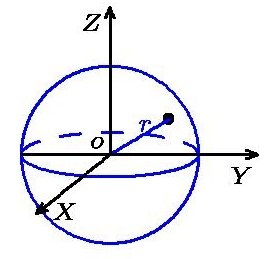
\includegraphics{bolanal.jpg}
\item[*] Cilindervlak met rotatieas de Z-as:\vskip 0.5cm
$\mathcal{C} \,\leftrightarrow\, x^2+y^2=r^2$\newline
%\docLink[tekening]{cilinderanal.jpg}{\includegraphics{tekening.gif}}
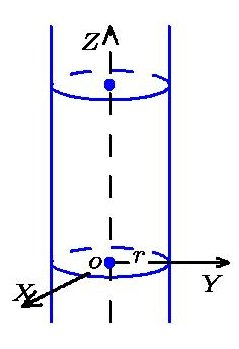
\includegraphics{cilinderanal.jpg}
\item[*] Kegelvlak met rotatieas de Z-as:\vskip 0.5cm
$\mathcal{K} \,\leftrightarrow\, x^2+y^2=(z-h)^2tg^2\alpha$\newline
%\docLink[tekening]{kegelanal.jpg}{\includegraphics{tekening.gif}}
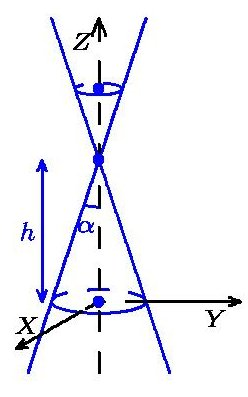
\includegraphics{kegelanal.jpg}
\item[*] Hyperbolo\"ide:\newline
\[\mathcal{H} \,\leftrightarrow\, x^2+y^2-z^2=1\]
\item[*] Parabolo\"ide:\newline
\[\mathcal{P}\, \leftrightarrow\, x^2+y^2=4z\]
%\includegraphics{para_klein.gif}
\end{itemize}


% Dit werk is gelicenseerd onder een Creative Commons
% Naamsvermelding-GelijkDelen 3.0 Unported.
% Bezoek http://creativecommons.org/licenses/by-sa/3.0/ om een kopie te zien 
% van de licentie of stuur een brief naar Creative Commons, 444 Castro Street, 
% Suite 900, Mountain View, California, 94041, USA.
